\subsection{Analyzing the corpus of regexes}
\label{sec:corpusAnalyzing}

\subsubsection{Studied feature set}

\begin{table*}[h!tb]
\centering
% \captionsetup{font=small}
\caption{Codes, descriptions and examples of select Python Regular Expression features}
\begin{small}
\label{table:featureDescriptions}
\begin{tabular}{l@{ }l@{ }l@{\hskip 0.37in} | l@{ }l@{ }l@{\hskip 0.37in}}
\textbf{Code} & \textbf{Description} & \textbf{Example} & \textbf{Code} & \textbf{Description} & \textbf{Example} \bigstrut \\
\noalign{\hrule height 0.08em}
\multicolumn{3}{c|}{Elements} & \multicolumn{3}{|c}{Operators} \bigstrut \\
\noalign{\hrule height 0.04em}
VWSP & matches U+000B & \begin{minipage}{0.5in}\begin{verbatim}\v\end{verbatim}\end{minipage} & ADD & one-or-more repetition & \begin{minipage}{0.5in}\begin{verbatim}z+\end{verbatim}\end{minipage}  \bigstrut \\
CCC & custom character class & \begin{minipage}{0.5in}\begin{verbatim}[aeiou]\end{verbatim}\end{minipage}  & KLE & zero-or-more repetition & \begin{minipage}{0.5in}\begin{verbatim}.*\end{verbatim}\end{minipage} \bigstrut \\
NCCC & negated CCC & \begin{minipage}{0.5in}\begin{verbatim}[^qwxf]\end{verbatim}\end{minipage}  &
QST & zero-or-one repetition & \begin{minipage}{0.5in}\begin{verbatim}z?\end{verbatim}\end{minipage} \bigstrut \\
RNG & chars within a range & \begin{minipage}{0.5in}\begin{verbatim}[a-z]\end{verbatim}\end{minipage}  & SNG & exactly n repetition & \begin{minipage}{0.5in}\begin{verbatim}z{8}\end{verbatim}\end{minipage}  \bigstrut \\
ANY & any non-newline char & \begin{minipage}{0.5in}\begin{verbatim}.\end{verbatim}\end{minipage}  & DBB & $n\le x \le m$ repetition & \begin{minipage}{0.5in}\begin{verbatim}z{3,8}\end{verbatim}\end{minipage}  \bigstrut \\
DEC & any of: 0123456789 & \begin{minipage}{0.5in}\begin{verbatim}\d\end{verbatim}\end{minipage}  &
LWB & at least n repetition & \begin{minipage}{0.5in}\begin{verbatim}z{15,}\end{verbatim}\end{minipage} \bigstrut \\
NDEC & any non-decimal & \begin{minipage}{0.5in}\begin{verbatim}\D\end{verbatim}\end{minipage}   &  LZY & as few reps as possible & \begin{minipage}{0.5in}\begin{verbatim}z+?\end{verbatim}\end{minipage}  \bigstrut \\
WRD & [a-zA-Z0-9\_] & \begin{minipage}{0.5in}\begin{verbatim}\w\end{verbatim}\end{minipage} &   OR & logical or & \begin{minipage}{0.5in}\begin{verbatim}a|b\end{verbatim}\end{minipage} \bigstrut \\
\cline{4-6}
NWRD & non-word chars & \begin{minipage}{0.5in}\begin{verbatim}\W\end{verbatim}\end{minipage}  &  \multicolumn{3}{|c}{Positions} \bigstrut \\
\cline{4-6}
WSP & \textbackslash t \textbackslash n \textbackslash r \textbackslash v \textbackslash f or space & \begin{minipage}{0.5in}\begin{verbatim}\s\end{verbatim}\end{minipage}   &  STR & start-of-line & \begin{minipage}{0.5in}\begin{verbatim}^\end{verbatim}\end{minipage} \bigstrut \\
NWSP & any non-whitespace & \begin{minipage}{0.5in}\begin{verbatim}\S\end{verbatim}\end{minipage}   & END & end-of-line & \begin{minipage}{0.5in}\begin{verbatim}$\end{verbatim}\end{minipage} \bigstrut \\
CG & a capture group & \begin{minipage}{0.5in}\begin{verbatim}(caught)\end{verbatim}\end{minipage}  & ENDZ & absolute end of string & \begin{minipage}{0.5in}\begin{verbatim}\Z\end{verbatim}\end{minipage} \bigstrut \\
BKR & match the $i^{th}$ CG & \begin{minipage}{0.5in}\begin{verbatim}\1\end{verbatim}\end{minipage} & WNW & word/non-word boundary & \begin{minipage}{0.5in}\begin{verbatim}\b\end{verbatim}\end{minipage} \bigstrut \\
PNG & named capture group & \begin{minipage}{0.5in}\begin{verbatim}(?P<name>x)\end{verbatim}\end{minipage}   &  NWNW & negated WNW & \begin{minipage}{0.5in}\begin{verbatim}\B\end{verbatim}\end{minipage} \bigstrut \\
BKRN & references PNG & \begin{minipage}{0.5in}\begin{verbatim}(P?=name)\end{verbatim}\end{minipage}  &   LKA & matching sequence follows & \begin{minipage}{0.5in}\begin{verbatim}a(?=bc)\end{verbatim}\end{minipage} \bigstrut \\
NCG & group without capturing & \begin{minipage}{0.5in}\begin{verbatim}a(?:b)c\end{verbatim}\end{minipage}   & LKB & matching sequence precedes & \begin{minipage}{0.5in}\begin{verbatim}(?<=a)bc\end{verbatim}\end{minipage} \bigstrut \\
\cline{1-3}
\multicolumn{3}{c|}{Options} & NLKA & sequence doesn't follow  & \begin{minipage}{0.5in}\begin{verbatim}a(?!yz)\end{verbatim}\end{minipage} \bigstrut \\
\cline{1-3}
OPT & options wrapper & \begin{minipage}{0.5in}\begin{verbatim}(?i)CasE\end{verbatim}\end{minipage}  & NLKB & sequence doesn't precede & \begin{minipage}{0.5in}\begin{verbatim}(?<!x)yz\end{verbatim}\end{minipage}  \bigstrut \\
\noalign{\hrule height 0.06em}
\end{tabular}
\end{small}
\vspace{-12pt}
\end{table*}


This thesis will focus on the features and syntax described in Table~\ref{table:featureDescriptions}.  Every regex in the corpus only uses features from this feature set.  A detailed introduction to the functionality of these features as studied in this thesis is provided in Section~\ref{sec:featureDescriptions}.  The features of Python Regular Expressions analyzed fall into four categories:

\begin{enumerate} \itemsep -1pt
\item{Elements are individual characters, character classes and logical groups.  Elements can be operated on by operators.}
\item{Options fundamentally modify the behavior of the engine.}
\item{Repetition modifiers, implicit concatenation and logical OR are operators. The order of operations is described in Section~\ref{sec:orderOfOperations}}.
\item{Positions refer to a position between characters.  They make assertions about the string on one or both sides of their position.}
\end{enumerate}

\subsubsection{Parsing feature tokens}
For each escaped pattern, the PCRE-parser produces a tree of feature tokens, which is converted to a vector by counting the number of each token in the tree.  For a simple example, consider the patterns in Figure~\ref{fig:featureParsing}.  The pattern \verb!"^m+(f(z)*)+"! contains four different types of tokens. It has the KLE operator (\verb!*!), the ADD operator (\verb!+!), two CG elements (\verb!(...)!), and the STR position (\verb!^!). A detailed description of all studied features is provided in Section~\ref{sec:featureDescriptions}.

\begin{figure}[hb]
\centering
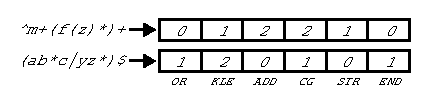
\includegraphics[height=0.6in]{nontex/illustrations/featureParsing.eps}
\caption{Two patterns parsed into feature vectors}
\label{fig:featureParsing}
\vspace{-12pt}
\end{figure}

Once all patterns were transformed into vectors, each feature was examined independently for all patterns, tracking the number of patterns, files and projects that the each feature appears in at least once.
